\noindent The code implementation of request from HTTP and analyze JSON is shown in Fig.\ref{png12}. It first use alamonfire to request from HTTP which include URL, method, parameters, encoding, headers and interceptor. When the system gets JSON database, it uses ObjectMapper to analyze the data and change it into a data array. It will also send to the view controller when the app receives a memory warning.

\begin{figure}[H]
  \centering
  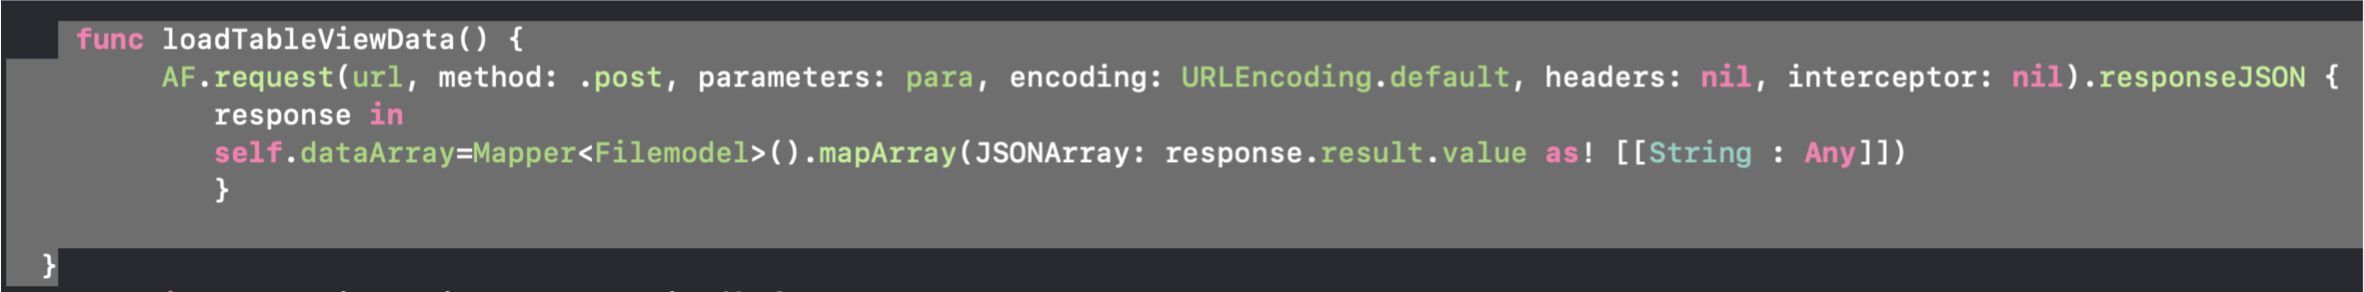
\includegraphics[width=.8\textwidth]{ios.png} %图片文件的相对路径
  \caption{Code snippet of request from HTTP and analyze JASON} %caption是图片的标题
  \label{png12} %此处的label相当于一个图片的专属标志,目的是方便上下文的引用
\end{figure}




\vspace{0.3cm}
\noindent This page \ref{pss} contains specific code about how to set the users authorities.
\begin{figure}[H]
  \centering
  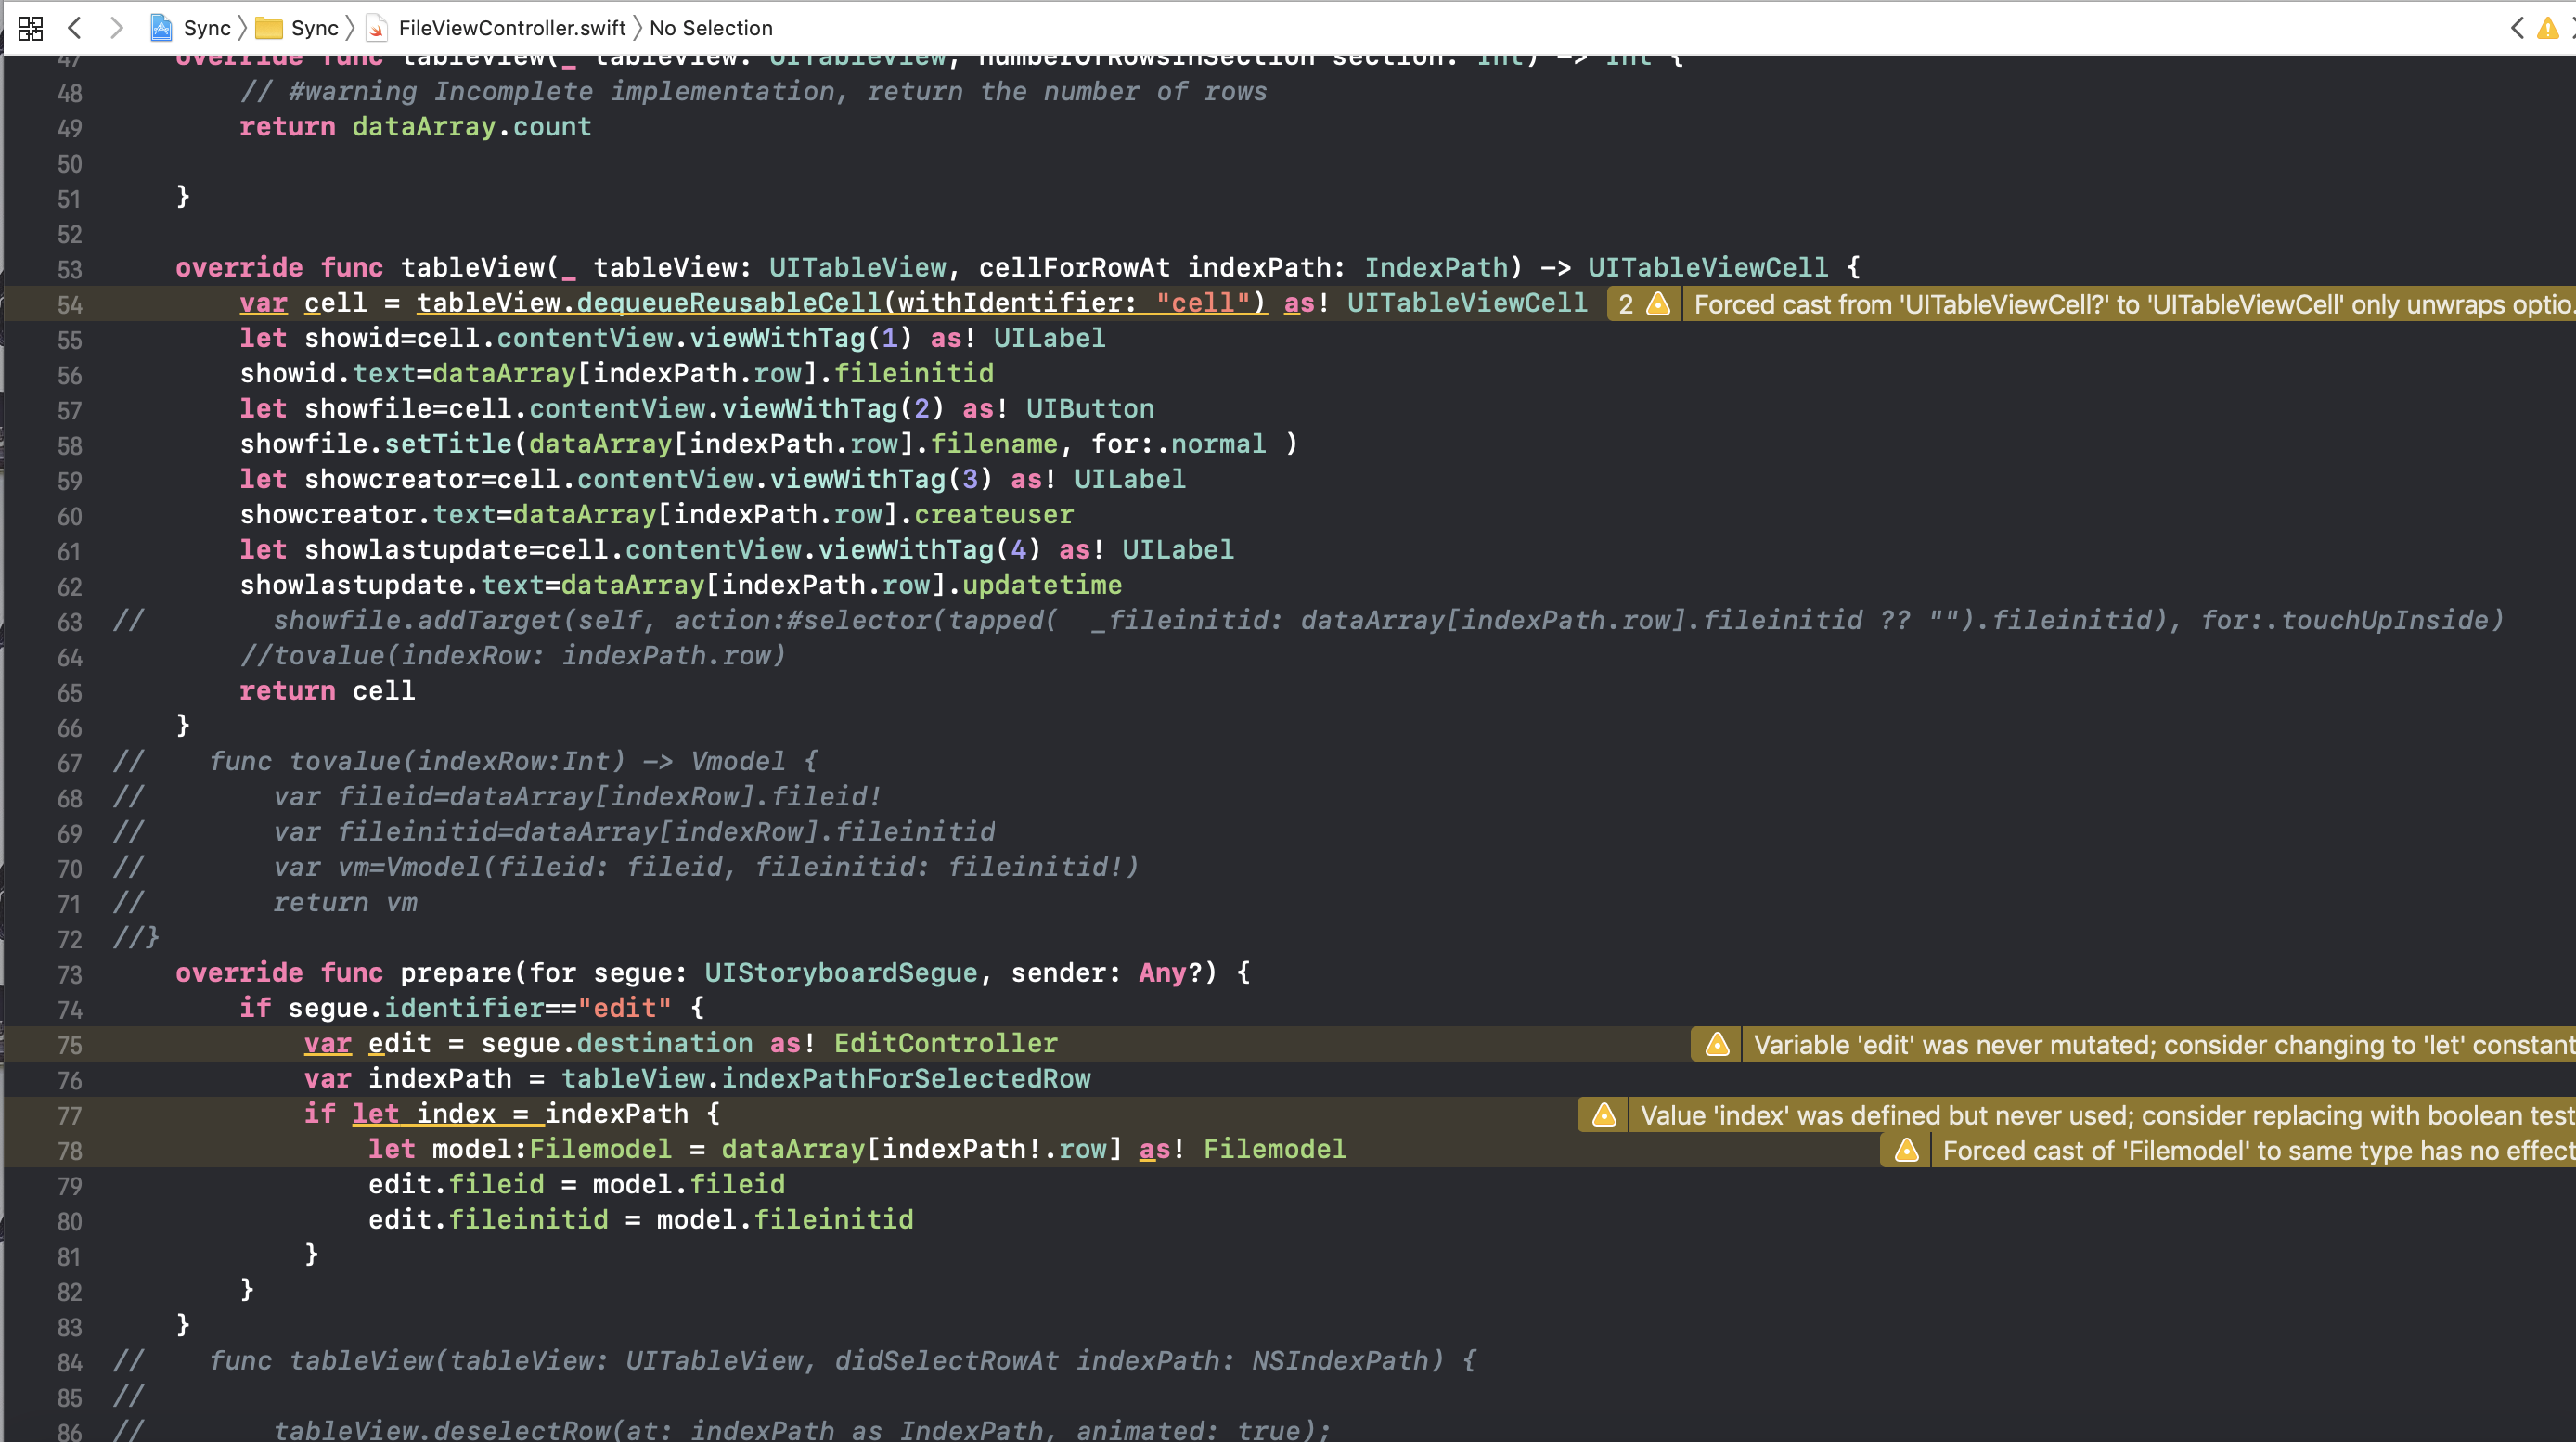
\includegraphics[width=.8\textwidth]{fv.png} %图片文件的相对路径
  \caption{Code snippet of set user authority} %caption是图片的标题
  \label{pss} %此处的label相当于一个图片的专属标志,目的是方便上下文的引用
\end{figure}

\vspace{0.3cm}
\noindent The code implementation of the Converting JSONArray and Model arrays using Object library is shown in Fig.\ref{ccc} and Fig.\ref{cc1}. These code use \texxxt{UITableView} to display a list of files and pass parameters between the view controller via \texxxt{segue}.
\begin{figure}[H]
  \centering
  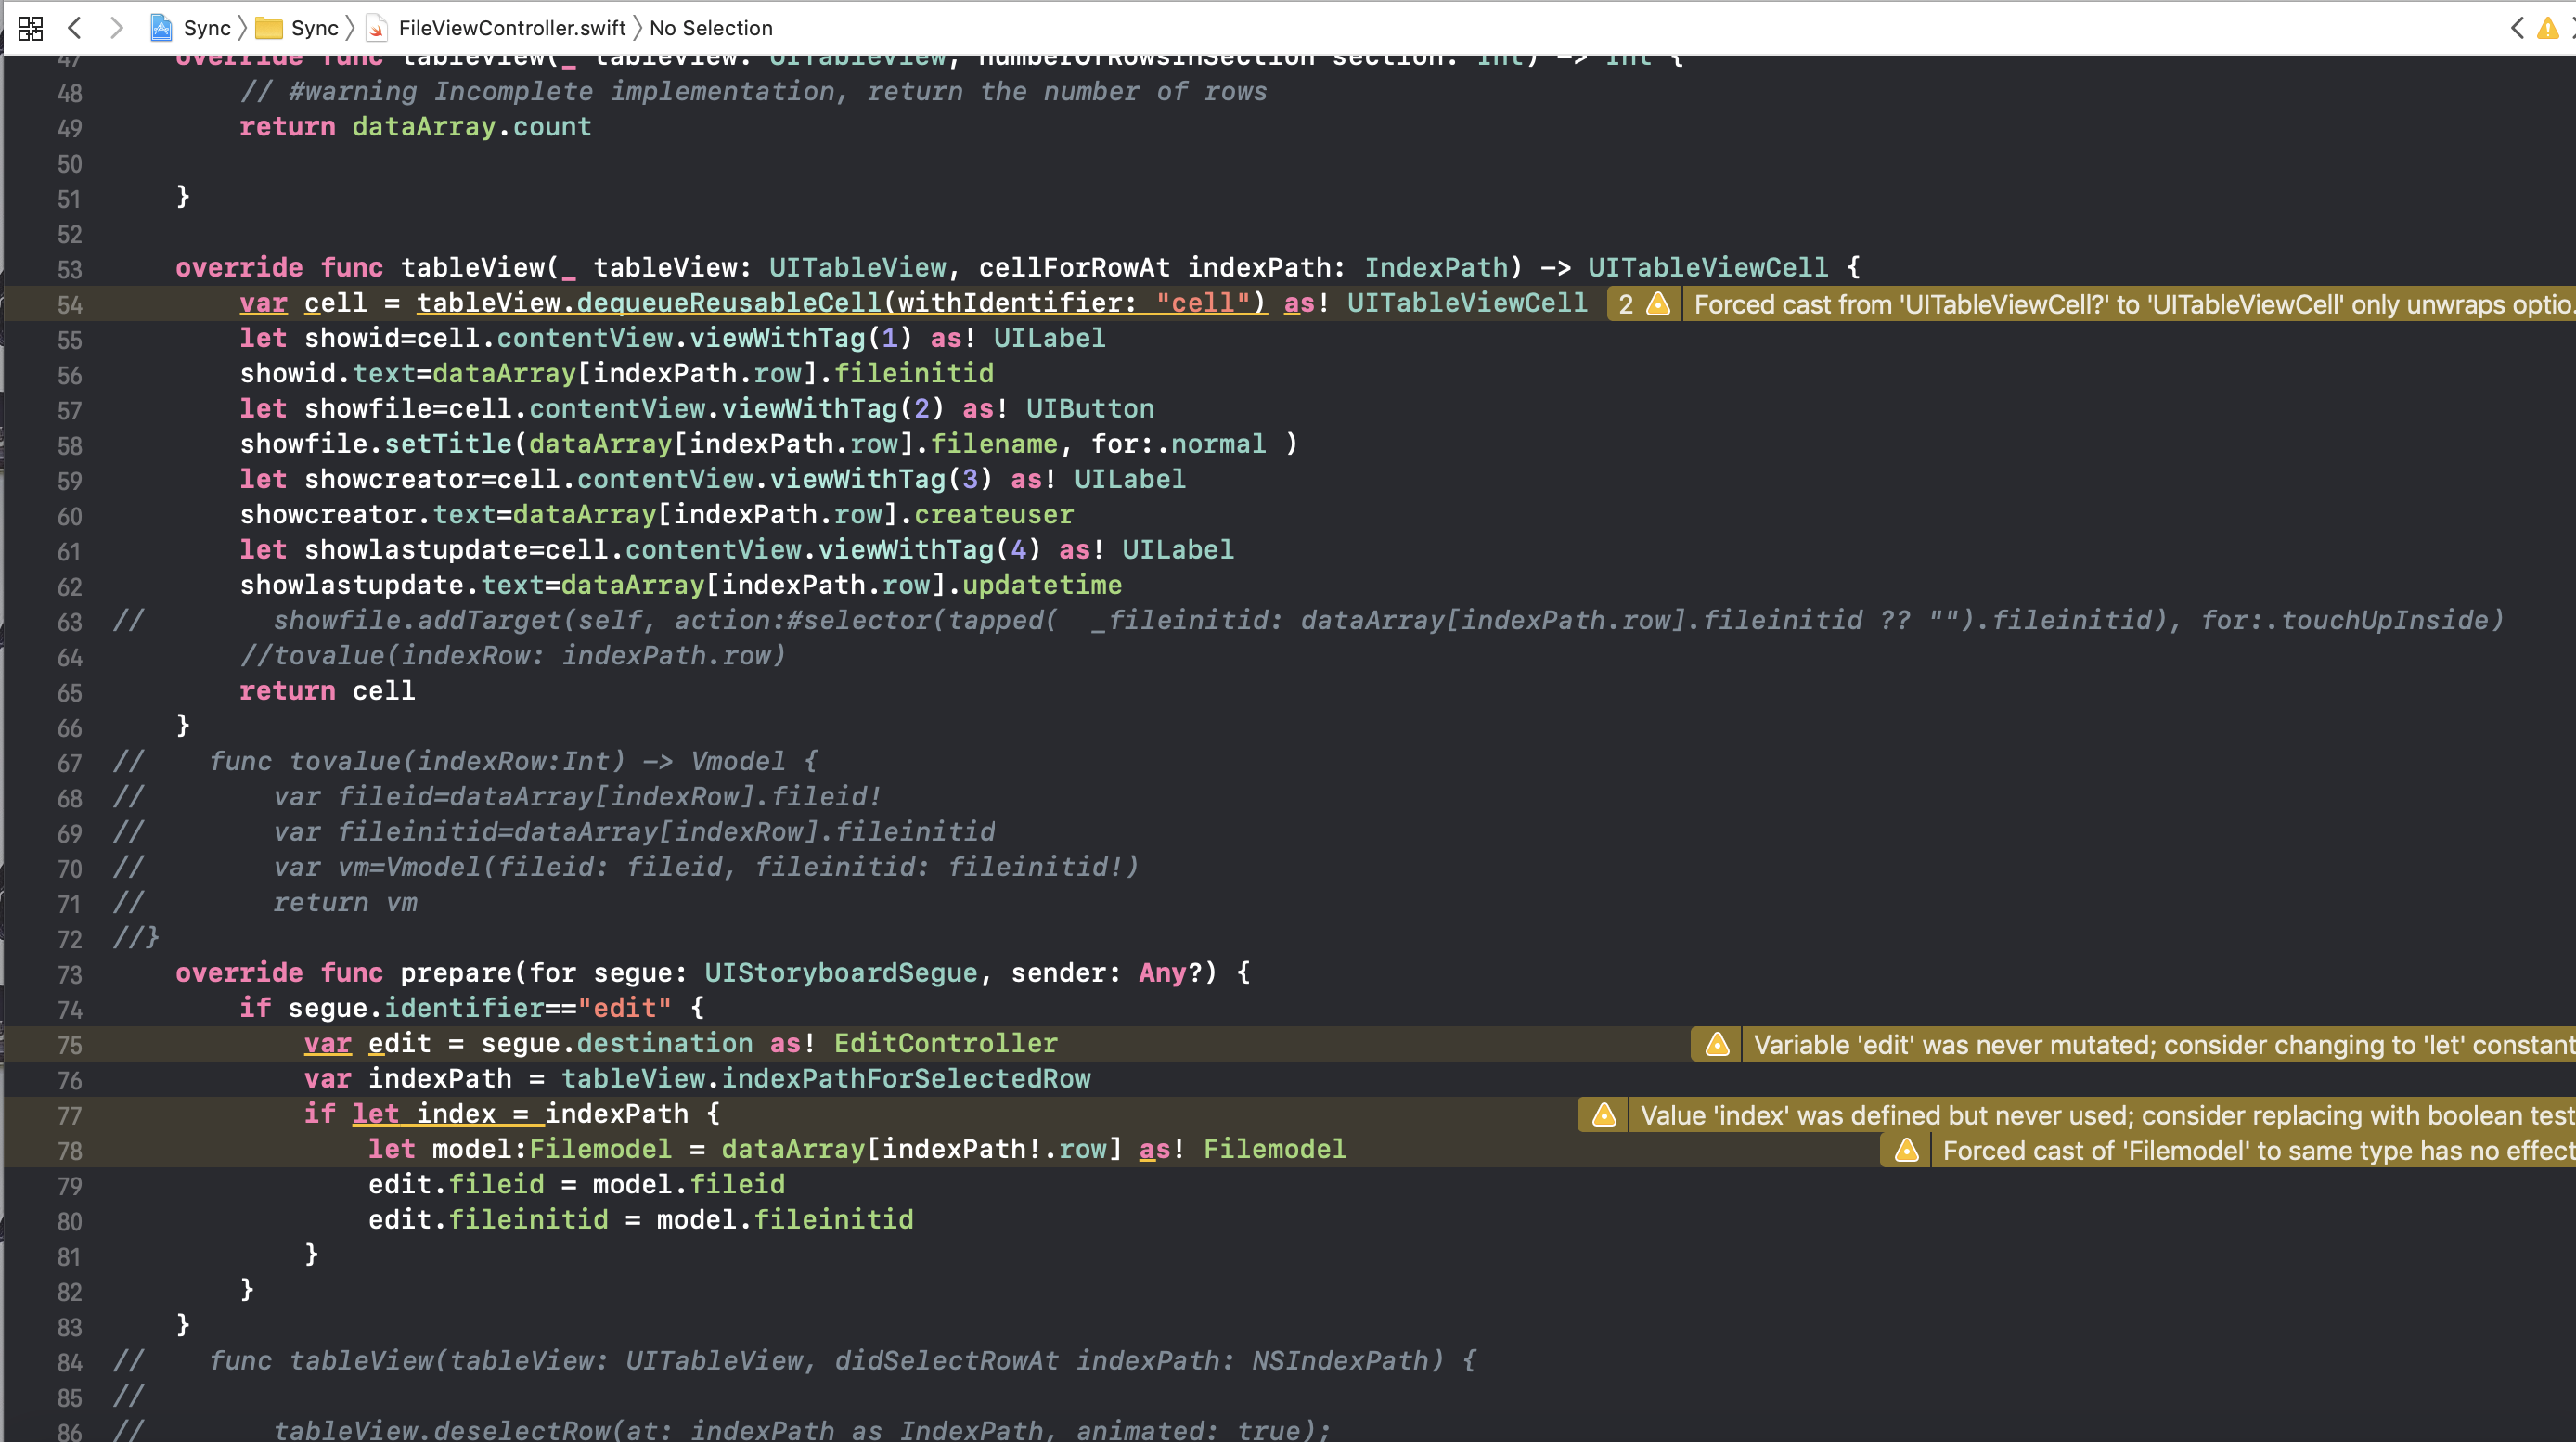
\includegraphics[width=.8\textwidth]{c1.png}%图片文件的相对路径
  \caption{Code snippet of Converting JSONArray and Model arrays} %caption是图片的标题
  \label{ccc} %此处的label相当于一个图片的专属标志,目的是方便上下文的引用
\end{figure}

\begin{figure}[H]
  \centering
  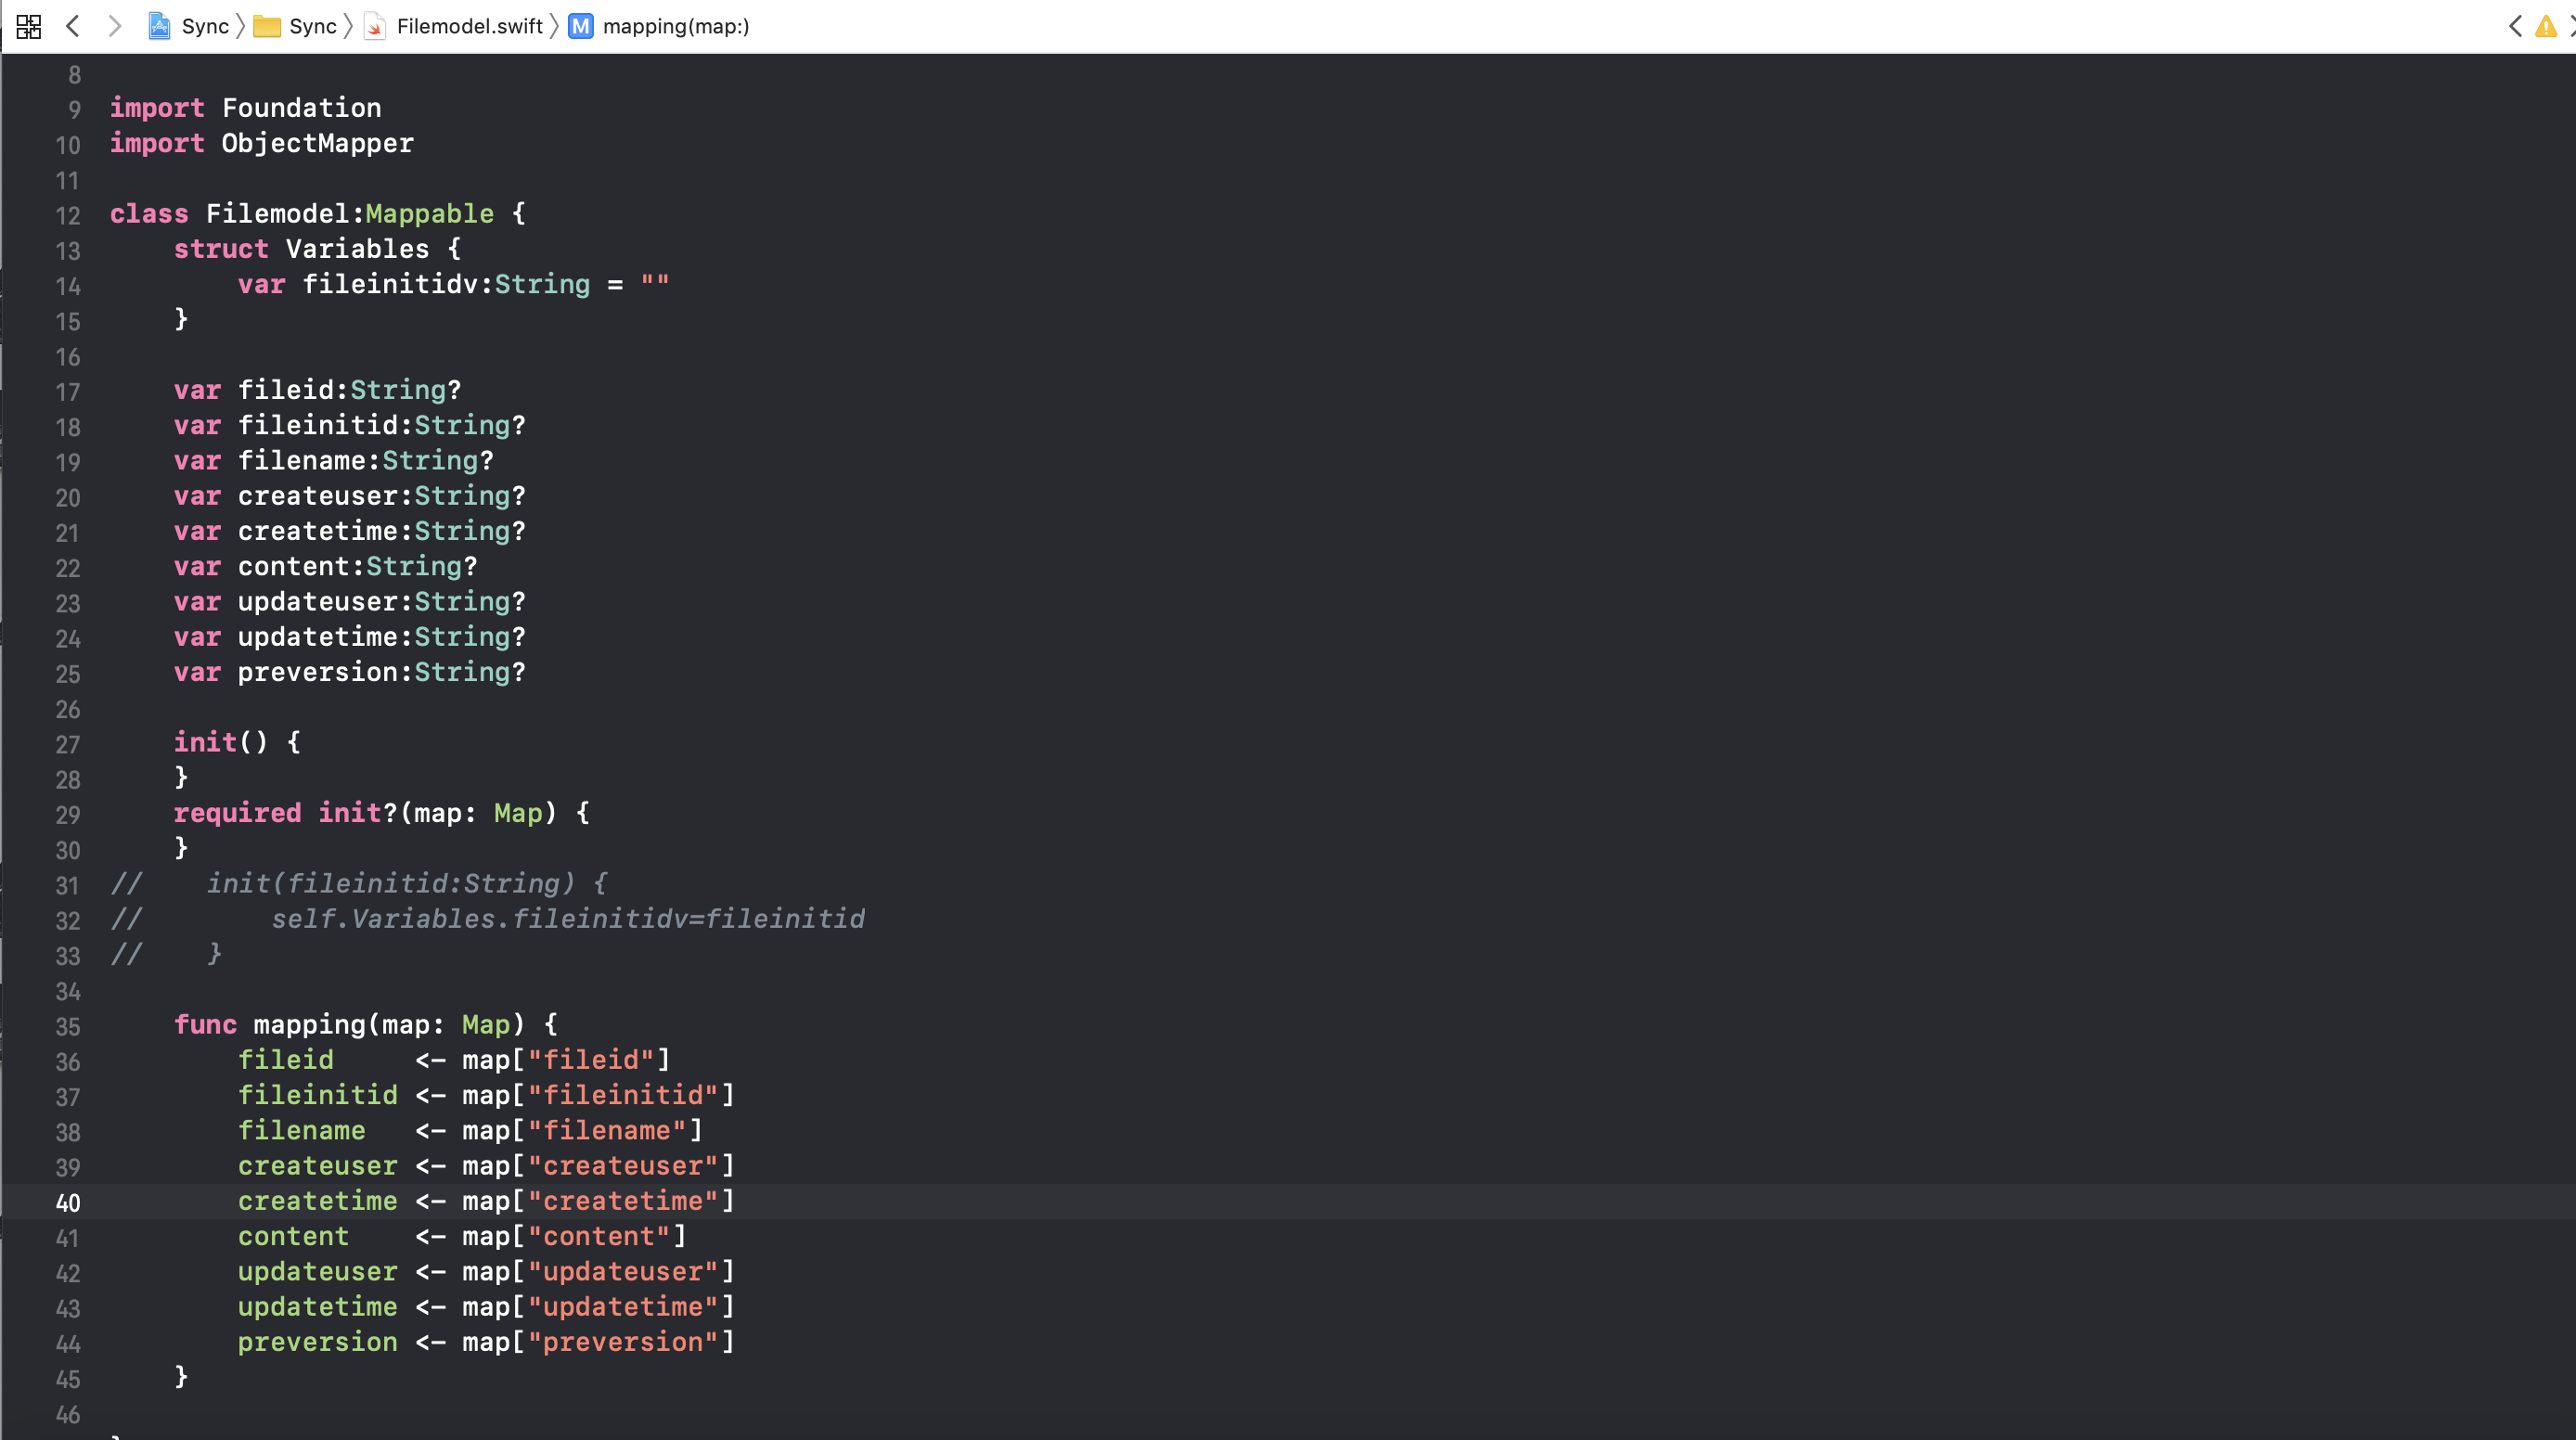
\includegraphics[width=.8\textwidth]{c2.png}%图片文件的相对路径
  \caption{Code snippet of Converting JSONArray and Model arrays} %caption是图片的标题
  \label{cc1} %此处的label相当于一个图片的专属标志,目的是方便上下文的引用
\end{figure}

\noindent The code implementation of returning data in the background is shown in Fig.\ref{aaa}. These code Use Just framework, which is an open source framework based on the Http NetWorking component, written in swift language to process http requests to exchange data with the background server, the background returns json-based bytes.
\begin{figure}[H]
  \centering
  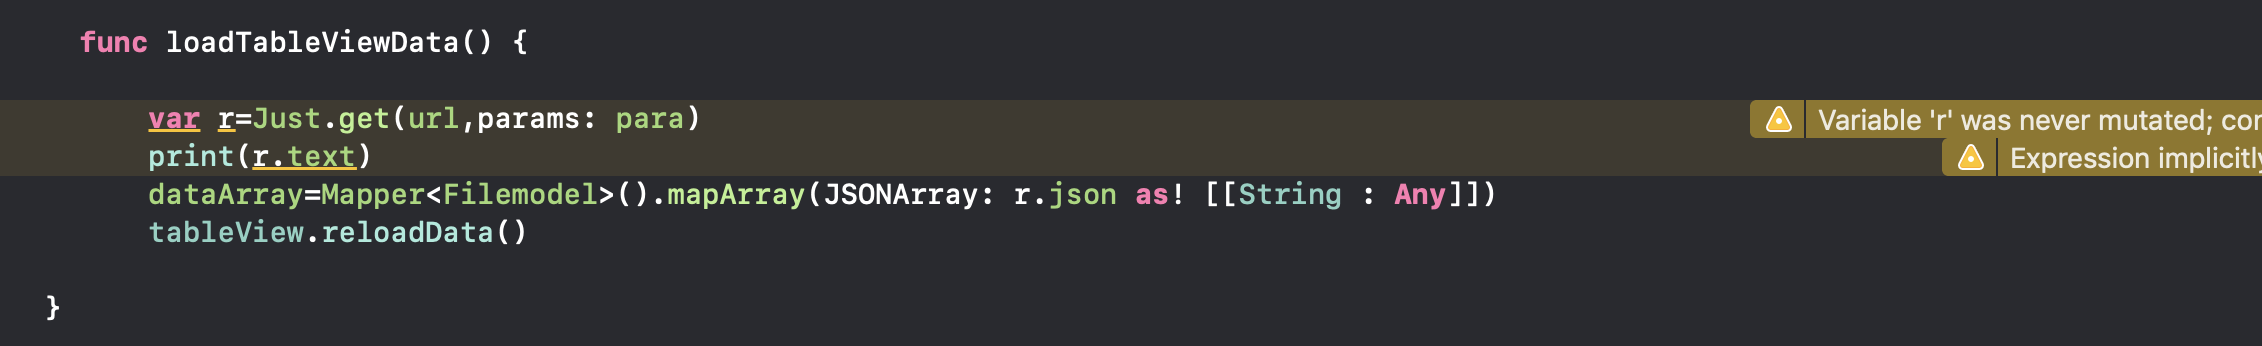
\includegraphics[width=.8\textwidth]{just.png}%图片文件的相对路径
  \caption{Code snippet of returning data in the background} %caption是图片的标题
  \label{aaa} %此处的label相当于一个图片的专属标志,目的是方便上下文的引用
\end{figure}

\vspace{0.3cm}
\noindent The code implementation of connecting database is shown in Fig.\ref{aa}.

\begin{figure}[H]
  \centering
  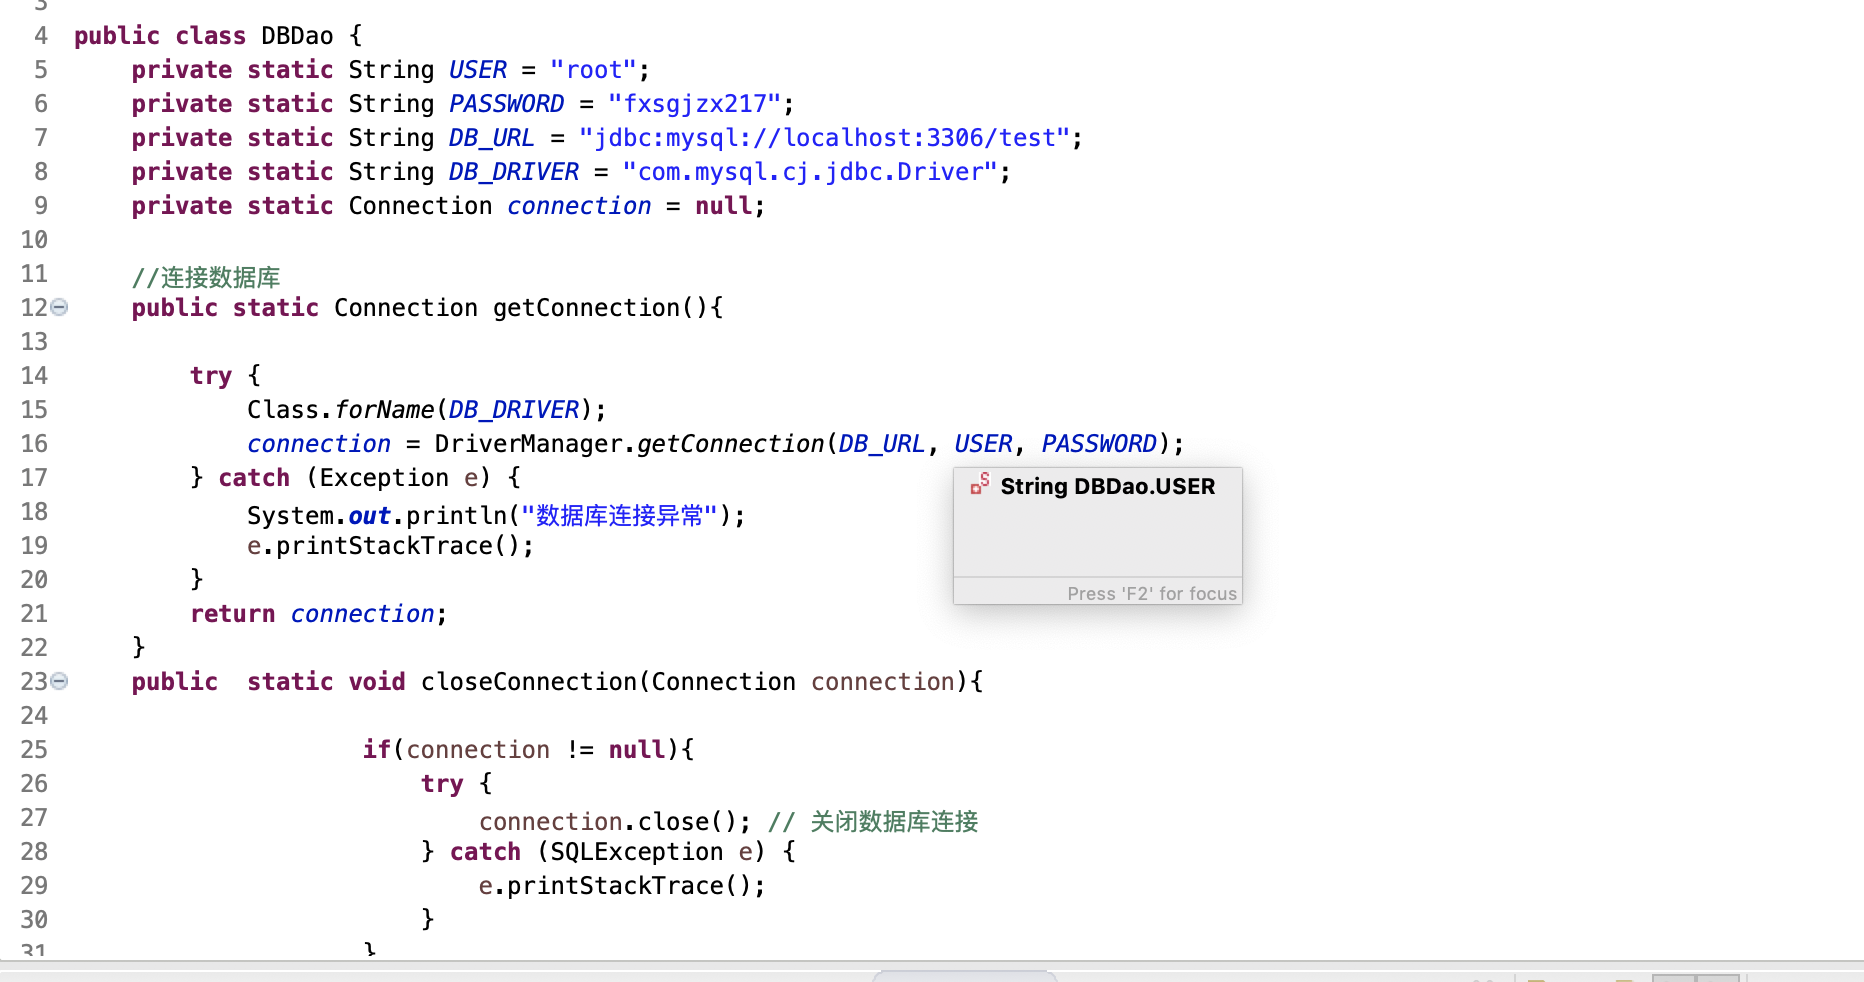
\includegraphics[width=.8\textwidth]{lianjie.png}%图片文件的相对路径
  \caption{Code snippet of Database linkage} %caption是图片的标题
  \label{aa} %此处的label相当于一个图片的专属标志,目的是方便上下文的引用
\end{figure}

\vspace{0.3cm}
\noindent The code implementation of how to get users information is shown in Fig.\ref{a1a}. It shows how to complete the settings and the acquisition of user information.

\begin{figure}[H]
  \centering
  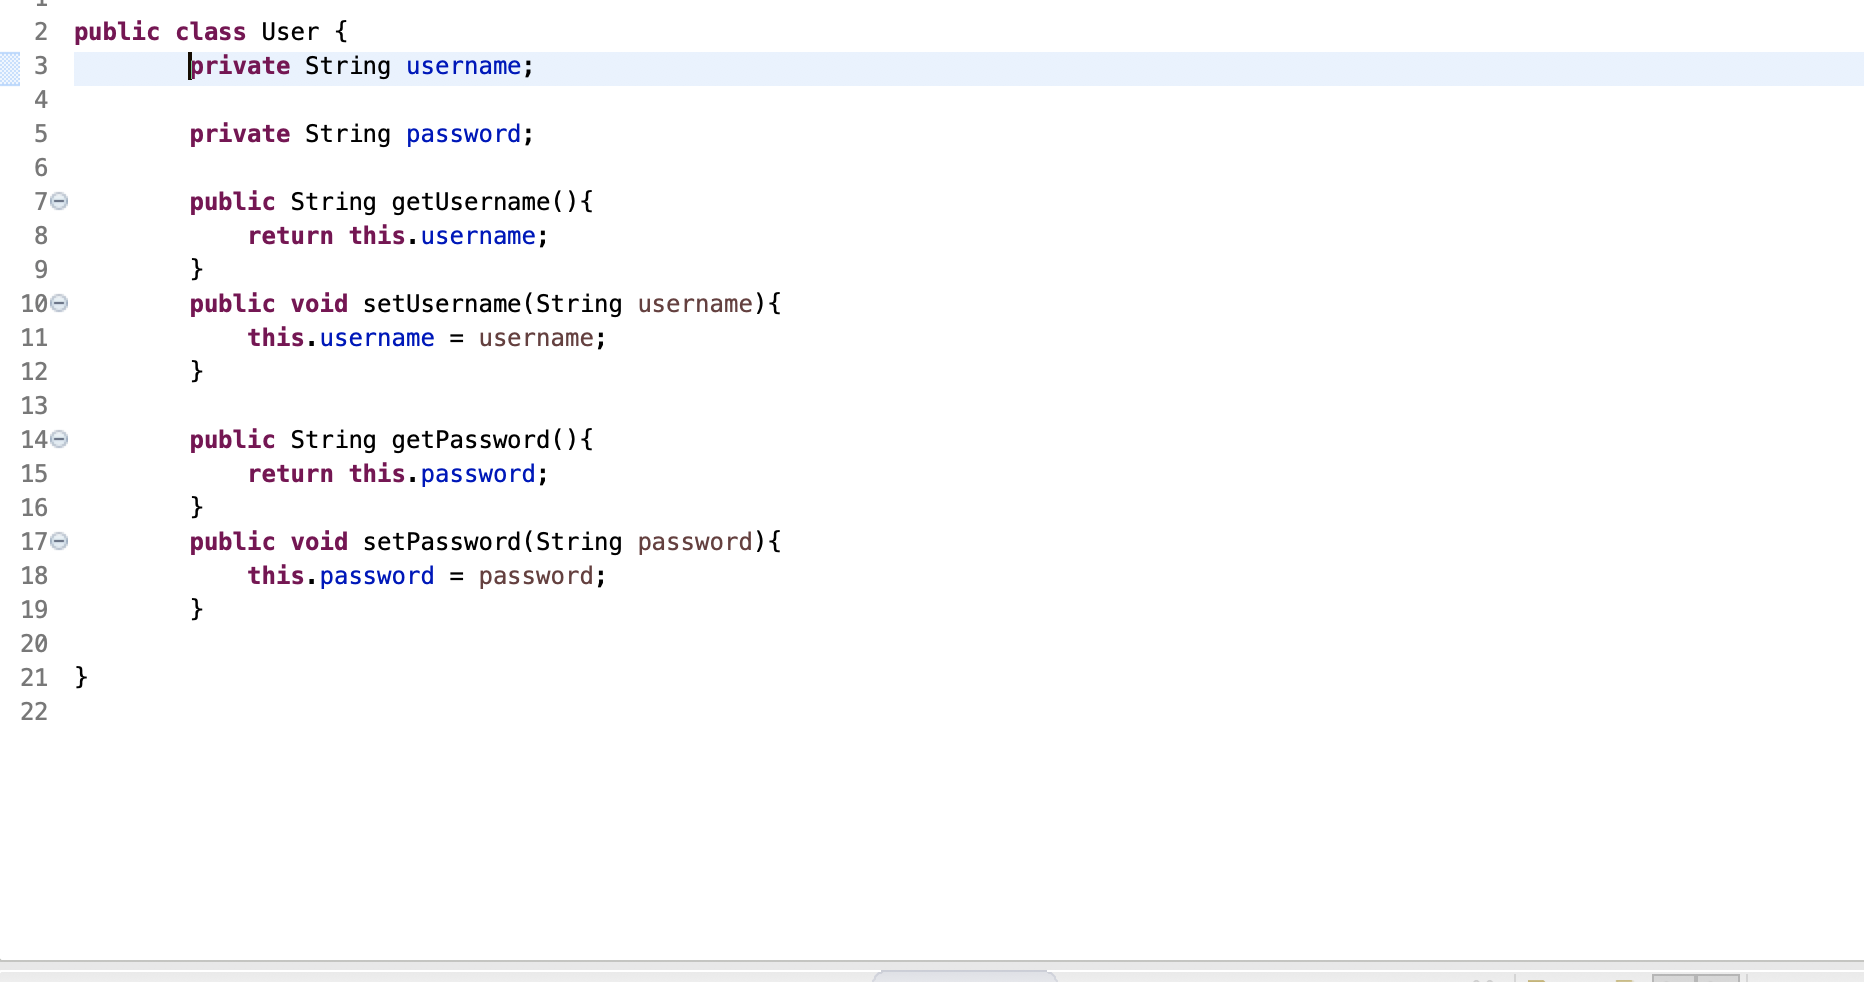
\includegraphics[width=.8\textwidth]{USERMODEL.png}%图片文件的相对路径
  \caption{Code snippet of the User Model} %caption是图片的标题
  \label{a1a} %此处的label相当于一个图片的专属标志,目的是方便上下文的引用
\end{figure}

\vspace{0.3cm}
\noindent The code implementation of how to compare file versions with \texttt{TestView} is shown in Fig.\ref{brian}. 

\begin{figure}[H]
  \centering
  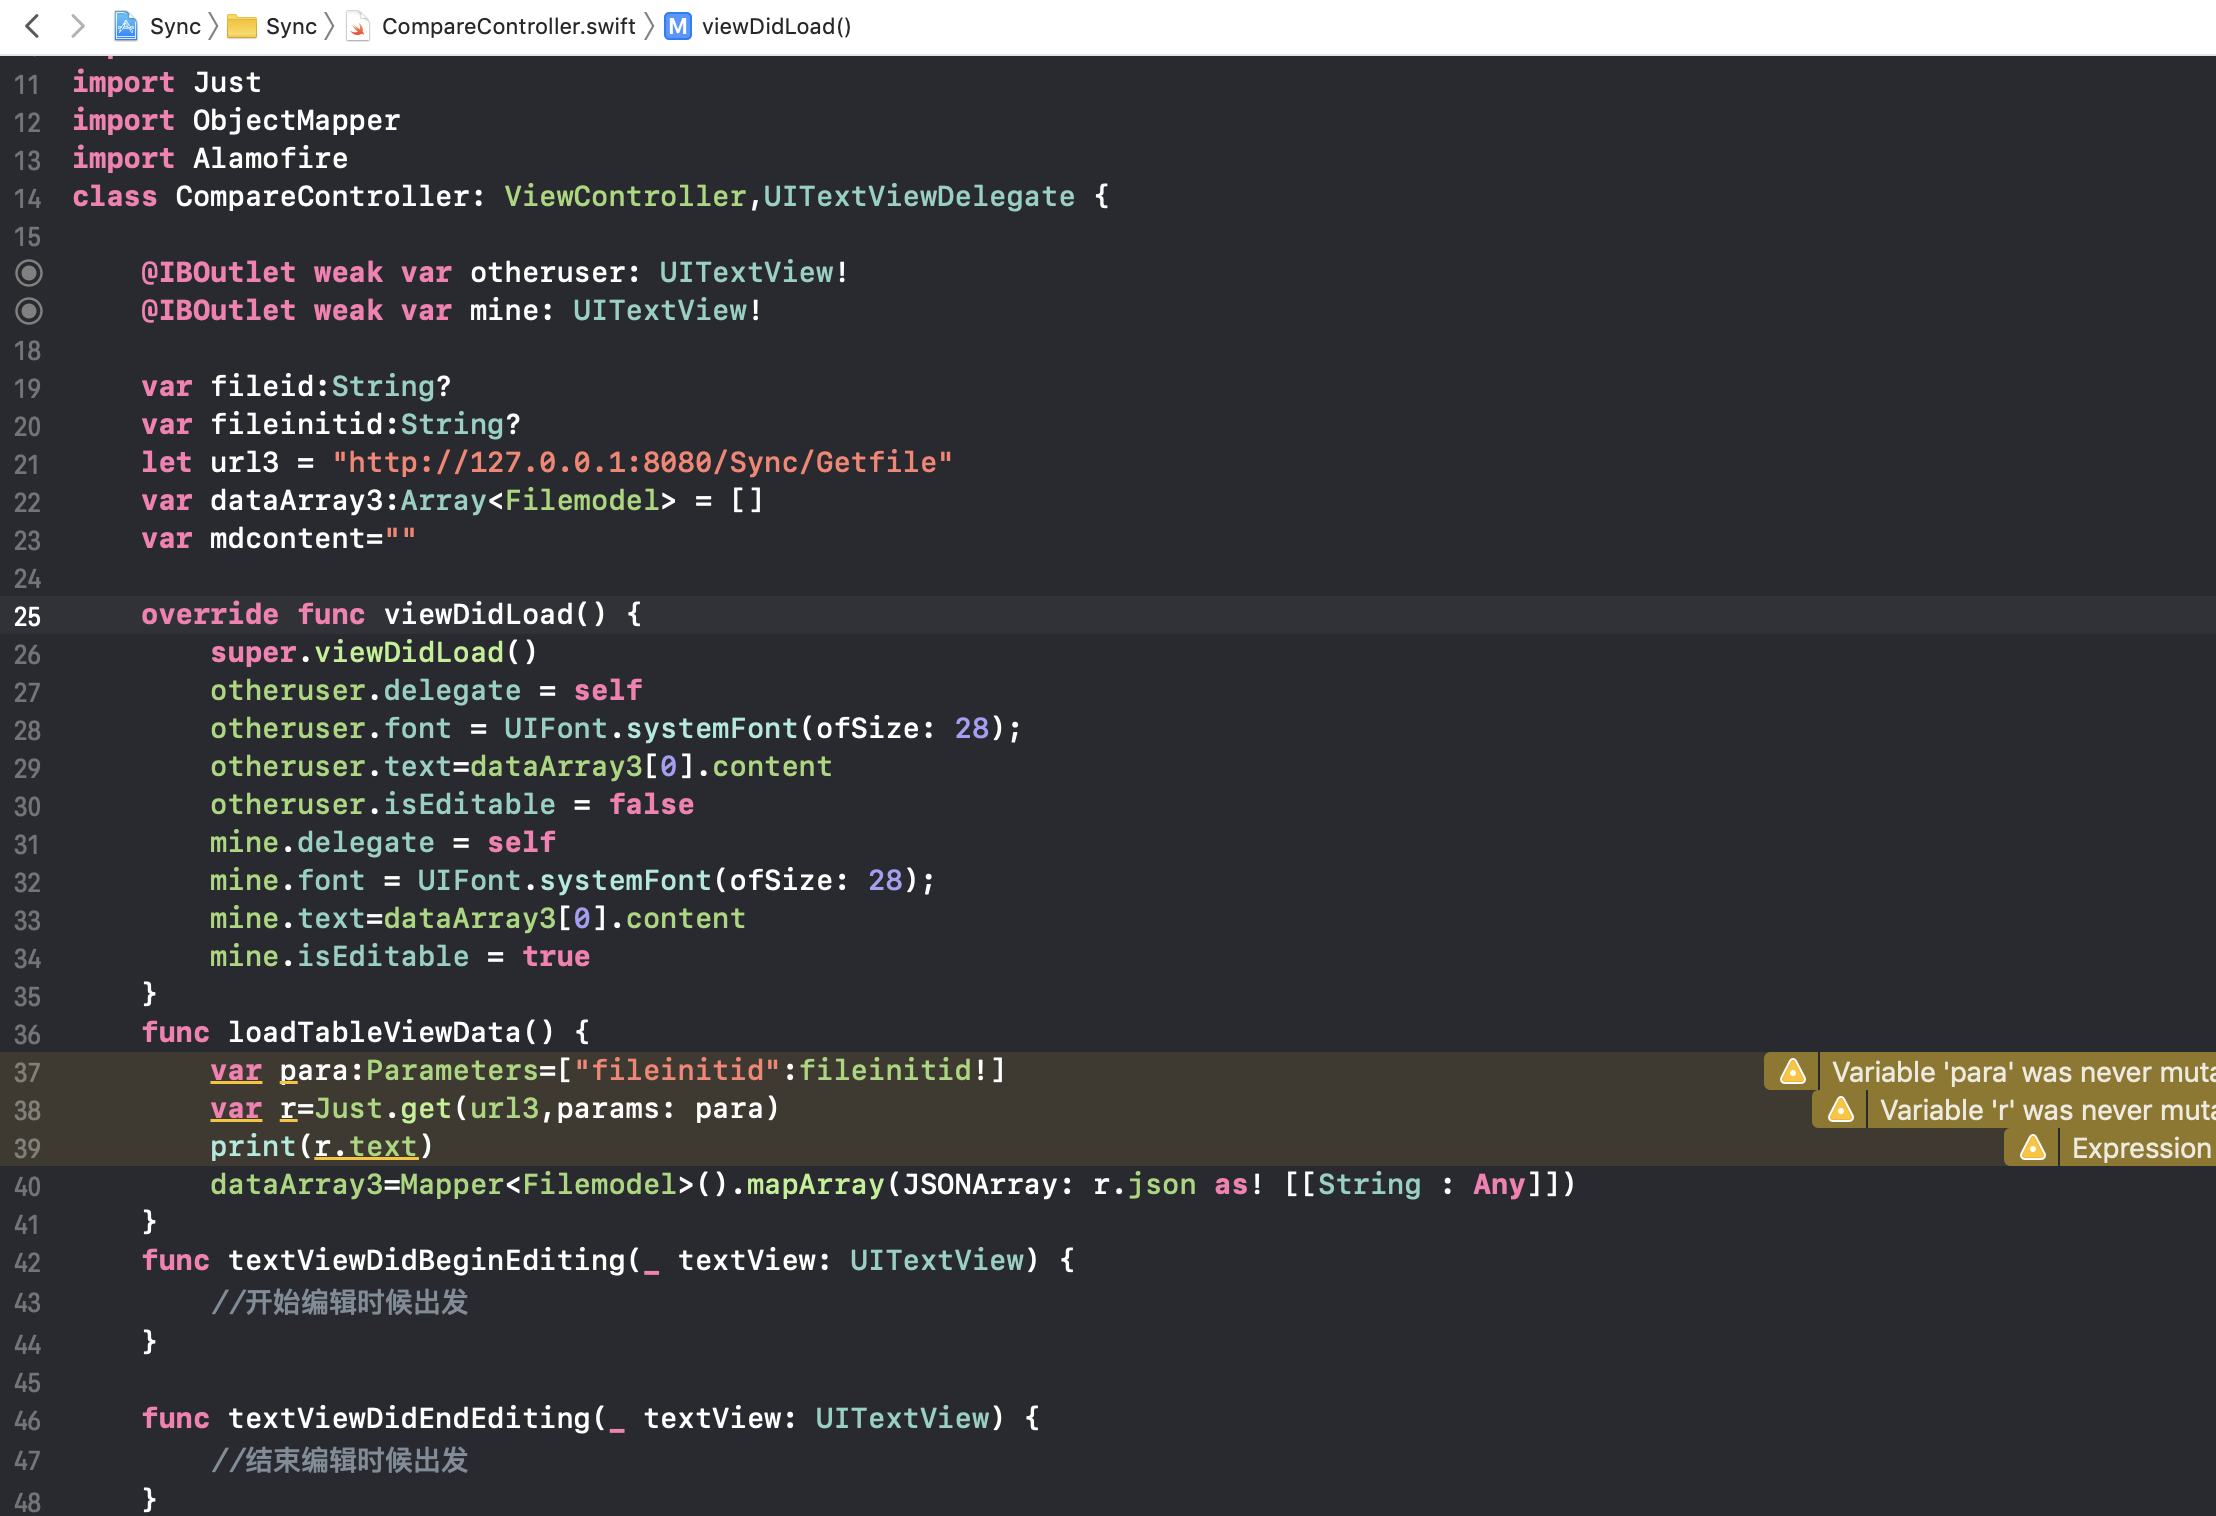
\includegraphics[width=.8\textwidth]{view.png}%图片文件的相对路径
  \caption{Code snippet of User Model} %caption是图片的标题
  \label{brian} %此处的label相当于一个图片的专属标志,目的是方便上下文的引用
\end{figure}

\vspace{0.3cm}
\noindent The code implementation of how to use SQL statements in this software is shown below. Fig.\ref{brian2} shows how to insert users information and file contents, and Fig.\ref{brian3} explains how to use SQL statements to query files according to their version number.

\begin{figure}[H]
  \centering
  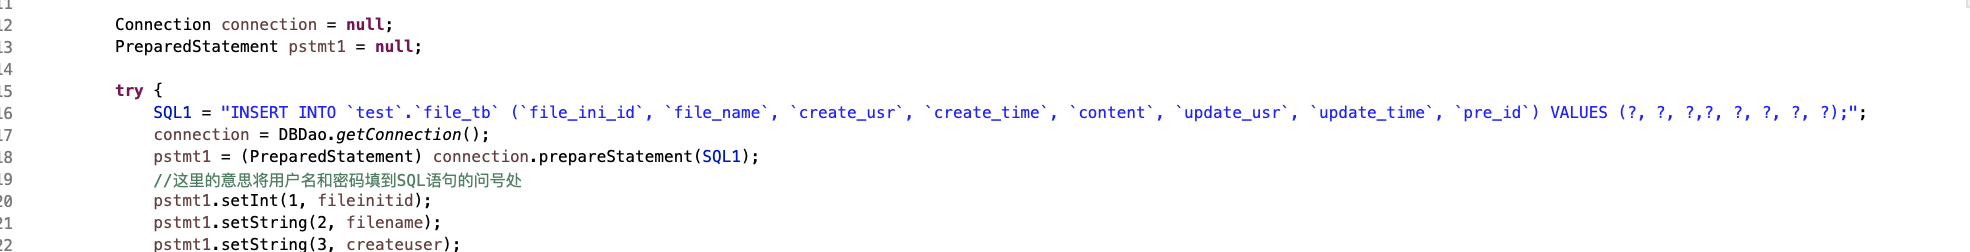
\includegraphics[width=.8\textwidth]{sql1.png}%图片文件的相对路径
  \caption{Code snippet of SQL statement 1} %caption是图片的标题
  \label{brian2} %此处的label相当于一个图片的专属标志,目的是方便上下文的引用
\end{figure}



\begin{figure}[H]
  \centering
  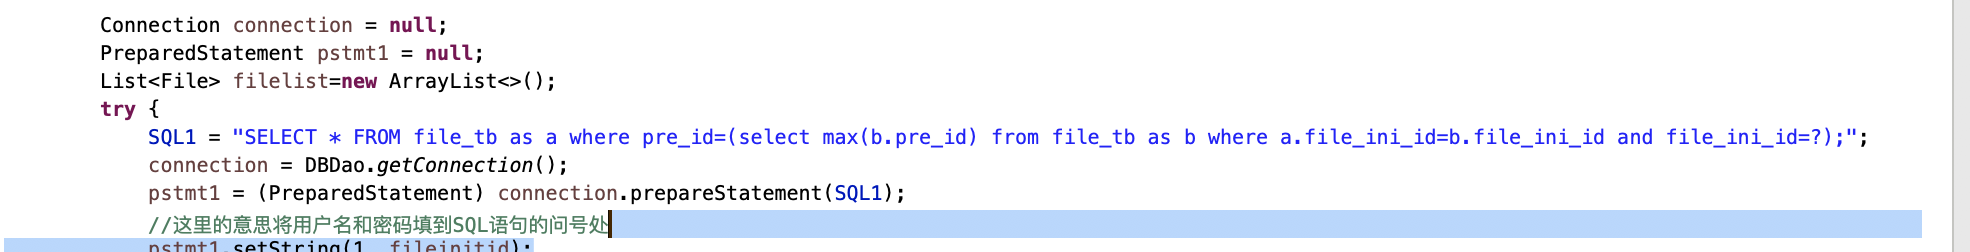
\includegraphics[width=.8\textwidth]{sql2.png}%图片文件的相对路径
  \caption{Code snippet of SQL statement 2} %caption是图片的标题
  \label{brian3} %此处的label相当于一个图片的专属标志,目的是方便上下文的引用
\end{figure}